%%%%%   TIPO DE DOCUMENTO: Artículo   %%%%%%
\documentclass[letterpaper,11pt,twoside]{report}

\usepackage[spanish]{babel} $%Idioma
\usepackage{graphicx} %Imágenes
\usepackage{float} % Paquete para forzar la posicion con [H]
\usepackage[utf8]{inputenc} %Acentos
\usepackage{hyperref} %Links
\usepackage{xspace}

\usepackage{listings}
\usepackage{verbatim}
\usepackage{amsmath, amssymb}
\usepackage{amsmath}
\usepackage[active]{srcltx}
\usepackage{amssymb}
\usepackage{amscd}
\usepackage{makeidx}
\usepackage{amsthm}
\usepackage{algpseudocode}
\usepackage{algorithm}
\renewcommand{\baselinestretch}{1}
\setcounter{page}{1}
\setlength{\textheight}{21.6cm}
\setlength{\textwidth}{14cm}
\setlength{\oddsidemargin}{1cm}
\setlength{\evensidemargin}{1cm}
\pagestyle{myheadings}
\thispagestyle{empty}
\markboth{\small{Tercera Actividad Técnica, Jorge Martinez.}}{\small{.}}
\date{}

\begin{document}
	\centerline{\bf Redes de Computadoras, \today}
	\centerline{}
	\begin{center}
		\Large{\textsc{Retardo de ida y vuelta: RTT}}
	\end{center}
	
	\centerline{}
	\centerline{\textbf{Martínez test Jorge Rafael}}
	\centerline{}
	
	\centerline{$correo, molap96@gmail.com$}
	
        \centerline{Universidad Aut\'onoma Metropolitana} 
	\centerline{Unidad Iztapalapa, M\'exico}
	
	\bigskip
	\section*{Experimentación con ping}

\noindent El primer paso para este experimento es escoger los destinos en otros continentes. Los destinos seleccionados son:

\begin{description}
	\item[Europa] IP de algún servidor de la Universidad Técnica de Berlín, Alemania (\emph{130.149.17.21})
	\item[Asia] IP de algún servidor de la Universidad de Tokio, Japón (\emph{133.11.11.11})
\end{description}

\begin{lstlisting}[language=Bash, caption=Pings con 300 muestras guardando la salida, label=lst:pings]
	ping -c 300 www.unam.mx > unam_full.dat
	ping -c 300 130.149.17.21 > alemania_full.dat
	ping -c 300 133.11.11.11 > tokio_full.dat
\end{lstlisting}

\noindent Ahora que tenemos los archivos con toda la informaci\'on de los ping es necesario extraer solo el valor num\'erico de estos. Para ello crearemos un script en AWK para poder obtener esta informaci\'on. 

\begin{figure}[H]
    \centering
    \begin{lstlisting}[frame=single, breaklines=true, basicstyle=\footnotesize\ttfamily, breakatwhitespace=false, columns=flexible, tabsize=2, showstringspaces=false, language=AWK] 
    {
        split($(NF-1), a, "="):
        print a[2]
    }
    \end{lstlisting}
    \caption{Script para extraer los datos requeridos}
    \label{fig:scriptAWK}
\end{figure}

El script funciona de la siguiente manera:


\begin{itemize}
    \item Para cada l\'inea del archivo, se extrae el pen\'utimo campo y lo divide en dos partes usando "=" como separador.
    \item Luego, imprime la segunda parte resultante de esta separaci\'on.
\end{itemize}

\noindent El siguiente paso es trazar por separado las tres gr\'aficas obtenidas. A continuaci\'on se muestran las tres gr\'aficas y las instrucciones en Octave para generarlas

\begin{figure}[H] 
    \centering 
    \begin{lstlisting}[frame=single, breaklines=true, basicstyle=\footnotesize\ttfamily, breakatwhitespace=false, columns=flexible, tabsize=2, showstringspaces=false, language=Octave] 
        load unam_RTT.dat 
        plot(unam_RTT, '--*', 'Color', 'k', 'LineWidth', 0.5, 'MarkerSize', 8) 
        grid on 
        xlabel ('Vuelta de transmision') 
        ylabel ('Ping [ms]') 
        title('Ping www.unam.mx') 
        print -dpng "trazaUnam.png" 
    \end{lstlisting} 
    \caption{Instrucciones para trazar la gr\'afica} 
    \label{fig:unamOctave} 
\end{figure}

\begin{figure}[H]
	\centering
	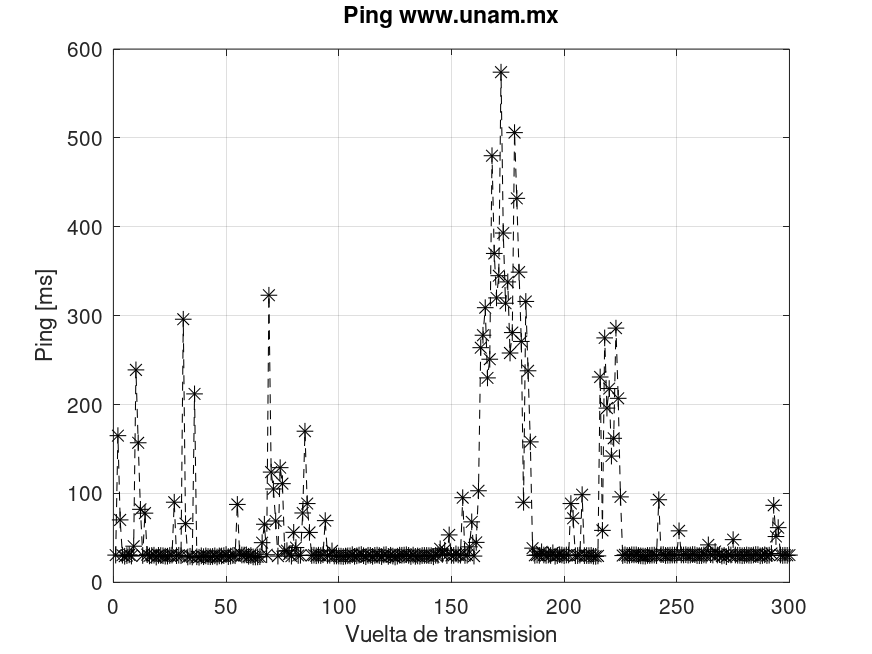
\includegraphics[width=0.90\textwidth]{img/trazaUnam.png}
	\caption{Gr\'afica de los datos del ping a www.unam.mx}
	\label{fig:unamGraph}
\end{figure}

\newpage

\begin{figure}[H] 
    \centering 
    \begin{lstlisting}[frame=single, breaklines=true, basicstyle=\footnotesize\ttfamily, breakatwhitespace=false, columns=flexible, tabsize=2, showstringspaces=false, language=Octave] 
        load alemania_RTT.dat 
        plot(alemania_RTT, '--*', 'Color', 'k', 'LineWidth', 0.5, 'MarkerSize', 8) 
        grid on 
        xlabel ('Vuelta de transmision') 
        ylabel ('Ping [ms]') 
        title('Ping 130.149.17.21') 
        print -dpng "trazaAlemania.png" 
    \end{lstlisting} 
    \caption{Instrucciones para trazar la gr\'afica} 
    \label{fig:alemaniaOctave} 
\end{figure}

\begin{figure}[H]
	\centering
	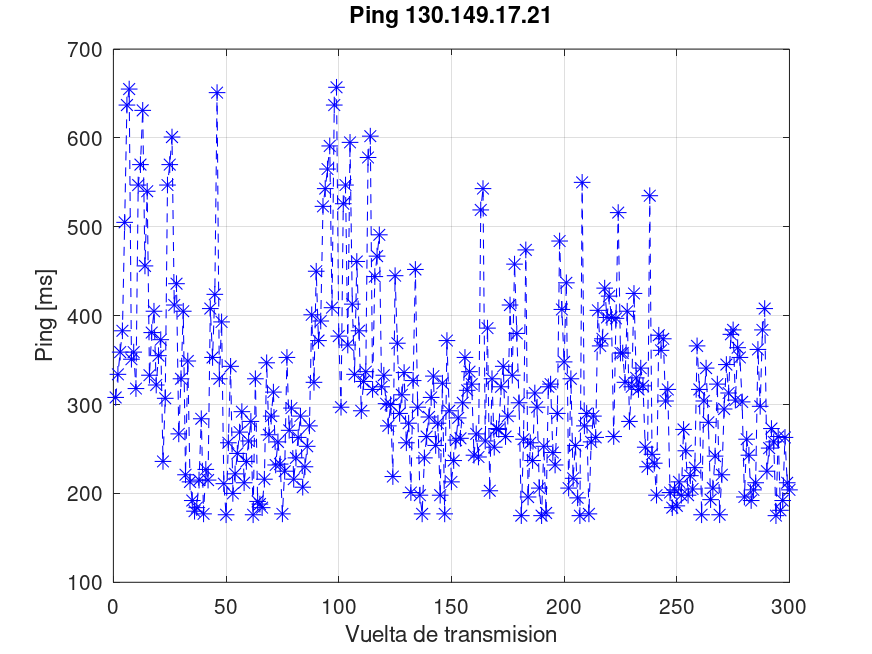
\includegraphics[width=0.90\textwidth]{img/trazaAlemania.png}
	\caption{Gr\'afica de los datos del ping a 130.149.17.21}
	\label{fig:alemaniaGraph}
\end{figure}

\newpage

\begin{figure}[H] 
    \centering 
    \begin{lstlisting}[frame=single, breaklines=true, basicstyle=\footnotesize\ttfamily, breakatwhitespace=false, columns=flexible, tabsize=2, showstringspaces=false, language=Octave] 
        load tokio_RTT.dat 
        plot(tokio_RTT, '--*', 'Color', 'k', 'LineWidth', 0.5, 'MarkerSize', 8) 
        grid on 
        xlabel ('Vuelta de transmision') 
        ylabel ('Ping [ms]') 
        title('Ping 133.11.11.11') 
        print -dpng "trazaTokio.png" 
    \end{lstlisting} 
    \caption{Instrucciones para trazar la gr\'afica} 
    \label{fig:tokioOctave} 
\end{figure}

\begin{figure}[H]
	\centering
	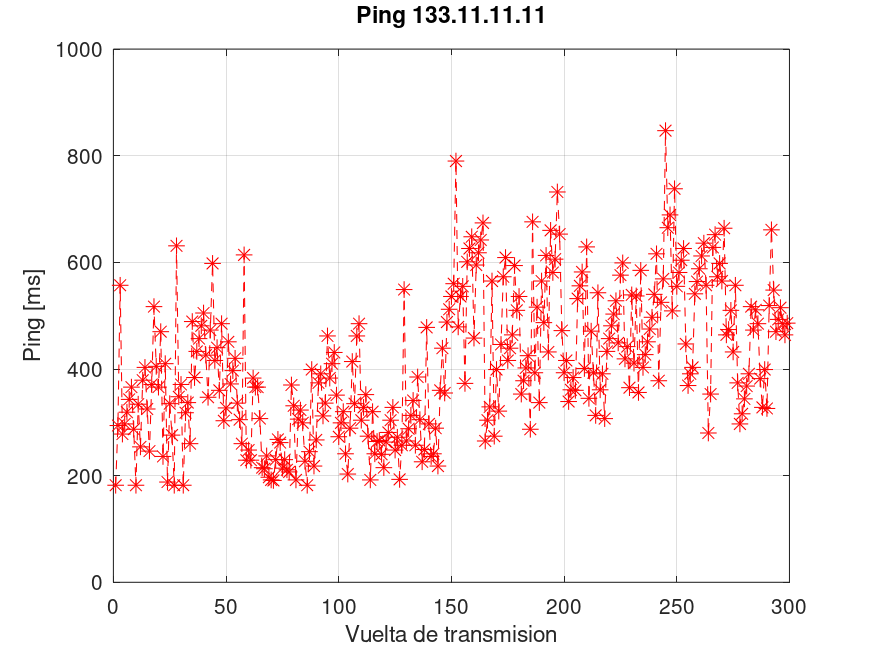
\includegraphics[width=0.90\textwidth]{img/trazaTokio.png}
	\caption{Gr\'afica de los datos del ping a 133.11.11.11}
	\label{fig:tokioGraph}
\end{figure}

\newpage
\noindent Recordando que el RTT (\emph{Round Trip Time}) es el tiempo que tarda una señal en viajar desde un punto a otro y regresar. Las gr\'aficas nos permiten ver como la distancia f\'isica entre los nodos influye significativamente en el RTT. A continuaci\'on se presentan algunos de los casos que se dan:

\begin{description}
    \item [Tiempo de propagaci\'on] - Cuanto mayor sea la distancia f\'isica, m\'as tiempo tardar\'a la señal en viajar, esto aumenta el tiempo de ida y vuelta.
    \item [Rutas alternativas] - Las longitudes mayores pueden obligar a tomar rutas alternativas que puedan tener diferentes carcter\'isticas de latencia.
    \item [Congesti\'o de nodos intermedios] - Los paquetes pueden pasar por m\'as nodos, aumentanto el riesgo de congesti\'on y retrasos adicionales.
    \item [Latenica adicional] - Cada nodo que un paquete atraviesa añade una pequeña cantidad de latencia, lo cual se acumula con mayor n\'umero de nodos.
\end{description}
	\section*{Experimentación con httping}
\end{document}